% An empty document to test the templates

\documentclass[compress]{beamer}
\usetheme{ninscwhite}

\usepackage{hyperref}
\hypersetup{linkcolor=blue} 

\title{Fundamentals of linear algebra}
\author{Germ{\'a}n G{\'o}mez-Herrero}
\institute{Advanced Human Neurophysiology\\VU University Amsterdam}
\date{\today}

%%%% Common mathematical definitions

%% Vectors and matrices
\def\q{{\mathbf q}}
\def\e{{\mathbf e}}
\def\m{{\mathbf m}}
\def\x{{\mathbf x}}
\def\X{{\mathbf X}}
\def\u{{\mathbf u}}
\def\U{{\mathbf U}}
\def\x{{\mathbf x}}
\def\z{{\mathbf z}}
\def\r{{\mathbf r}}
\def\h{{\mathbf h}}
\def\n{{\mathbf n}}
\def\cc{{\mathbf c}}
\def\s{{\mathbf s}}
\def\v{{\mathbf v}}
\def\j{{\mathbf j}}
\def\A{{\mathbf A}}
\def\y{{\mathbf y}}
\def\W{{\mathbf W}}
\def\H{{\mathbf H}}
\def\K{{\mathbf K}}
\def\w{{\mathbf w}}
\def\B{{\mathbf B}}
\def\G{{\mathbf G}}
\def\K{{\mathbf K}}
\def\N{{\mathbf N}}
\def\S{{\mathbf S}}
\def\Thetam{{\boldsymbol{\Thetam}}}
\def\Sigmam{{\boldsymbol{\Sigma}}}
\def\Phim{{\boldsymbol{\Phi}}}
\def\Omegam{{\boldsymbol{\Omega}}}
\def\Gammam{{\boldsymbol{\Gamma}}}
\def\Psim{{\boldsymbol{\Psi}}}
\def\psiv{{\boldsymbol{\psi}}}
\def\Pim{{\boldsymbol{\Pi}}}
\def\phiv{{\boldsymbol{\phi}}}
\def\omegav{{\boldsymbol{\omega}}}
\def\etav{{\boldsymbol{\eta}}}
\def\epsilonv{{\boldsymbol{\epsilon}}}
\def\mPsim{{\bar{\Psim}}}
\def\mpsi{{\bar{\psi}}}
\def\a{{\mathbf a}}
\def\b{{\mathbf b}}
\def\w{{\mathbf w}}
\def\D{{\mathbf D}}
\def\P{{\mathbf P}}
\def\n{{\mathbf n}}
\def\V{{\mathbf V}}
\def\R{{\mathbf R}}
\def\I{{\mathbf I}}
\def\M{{\mathbf M}}
\def\T{{\mathbf T}}
\def\C{{\mathbf C}}
\def\a{{\mathbf a}}
\def\b{{\mathbf b}}
\def\cv{{\mathbf c}}
\def\r{{\mathbf r}}
\def\x{{\mathbf x}}
\def\d{{\mathbf d}}
\def\v{{\mathbf v}}
\def\X{{\mathbf X}}
\def\Sigmam{{\boldsymbol{\Sigma}}} 
\def\muv{{\boldsymbol{\mu}}} 
\def\C{{\mathbf C}} 
\def\R{{\mathbf R}} 
\def\E{{\textrm E}} 
\def\A{{\mathbf A}}
\def\B{{\mathbf B}}
\def\W{{\mathbf W}}
\def\P{{\mathbf P}}
\def\bLambda{{\boldsymbol{\Lambda}}}
\def\bSigma{{\boldsymbol{\Sigma}}}
\def\E{{\vec{\mathbf E}}}
\def\Q{{\vec{\mathbf Q}}}

%% Numeric sets
\def\L{{\cal L}}
\def\cC{\mathcal{C}}
\def\cS{\mathcal{S}}
\def\cL{\mathcal{L}}

%% Operators
\def\sech{{\mathrm{sech}}}
\def\Cum{{\rm{Cum}}}
\def\var{{\rm{var}}}

\newcommand{\black}[1]{{\color{black}#1}}
\renewcommand{\emph}[1]{\textbf{\black{#1}}}
\newcommand{\beq}[1]{\[\black{#1}\]}
\renewcommand{\cv}{\black{\mathbf{c}}}
\renewcommand{\d}{\black{\mathbf{d}}}
\renewcommand{\v}{\black{\mathbf{v}}}

\begin{document}


\frame{
	\titlepage 
}


%%%%%%%%%%%%%%%%%%%%%%% SOLVING LINEAR EQUATIONS

\section{Linear equations}
\subsection*{}


\begin{frame}
\frametitle{The fundamental problem of linear algebra}

To solve $n$ linear equations in $n$ unknowns:

\beq{
\begin{array}{ccc}
2x - y & = & 0\\
-x + 2y& = &3
\end{array}
}

For $n=2$, solving by \emph{elimination} is easy:

\beq{
\left.\begin{array}{ccccc}
2x - y & = & 0 &\Rightarrow& y = 2x\\
-x + 2y& = &3&&
\end{array}\right\} -x + 2(2x) = 3 \Rightarrow 
\left\{
\begin{array}{ccc}x&=&1\\y&=&2\end{array}
\right.
}

\end{frame}

%%%%%%%%%%%%%%%%%%

\begin{frame}
\frametitle{The geometry of linear equations}
\framesubtitle{Row picture}

\begin{columns}
\column{.5\textwidth}
\begin{center}
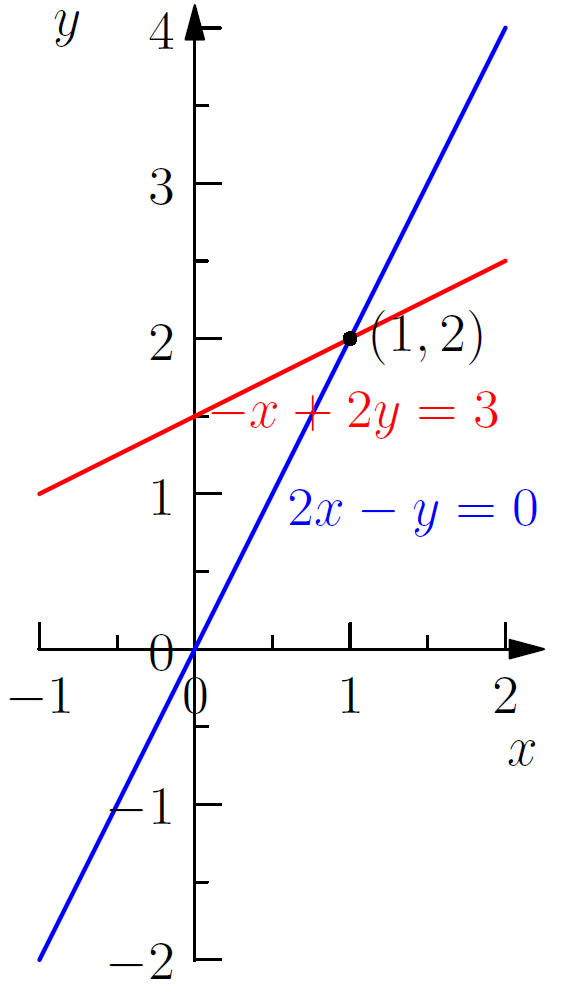
\includegraphics[trim = 5mm 5mm 5mm 1mm, clip, width=.6\textwidth]{./img/row-pic}
\end{center}
\column{.5\textwidth}
\begin{itemize}
\item The set of all valid solutions to a linear equation with $2$ unknowns defines a line in a 2-dimensional space
\vspace{.2cm}
\item The common solution to $m$ linear equations must be in the intersection between the $m$ lines that such equations define
\end{itemize}
\end{columns}

\end{frame}

%%%%%%%%%%%%%%%%%%

\begin{frame}
\frametitle{The geometry of linear equations}
\framesubtitle{Column picture}

\begin{columns}
\column{.5\textwidth}
\begin{center}
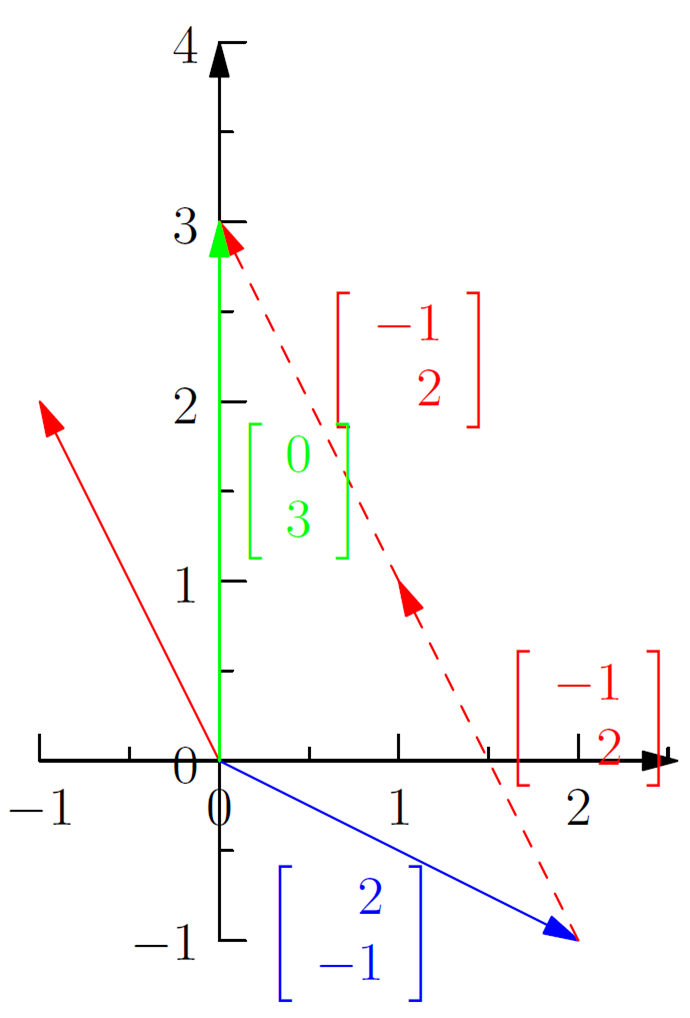
\includegraphics[trim = 2mm 2mm 2mm 2mm, clip, width=.7\textwidth]{./img/col-pic}
\end{center}

\column{.5\textwidth}
\beq{
x\underbrace{\left[
\begin{array}{r}
2\\-1
\end{array}
\right]}_{\cv}+
y\underbrace{\left[
\begin{array}{r}
-1\\2
\end{array}
\right]}_{\d}=
\underbrace{\left[
\begin{array}{r}
0\\3
\end{array}
\right]}_{v}
}

In \emph{vector} notation:

\beq{
x\cv + y\d = \v
}

\end{columns}

\vspace{.5cm}
Vector $\v$ is a \emph{linear combination} of vectors $\cv$ and $\d$, and $\black{x=1}$, $\black{y=2}$ are the linear combination \emph{coefficients}.

\end{frame}


%%%%%%%%%%%%%%%%%%

\begin{frame}
\frametitle{A simple exercise}

How many \black{unknowns} (aka variables, aka coefficients)?

\vspace{.2cm}

How many \black{equations}?

\vspace{.2cm}

How many \black{solutions}?

\begin{center}
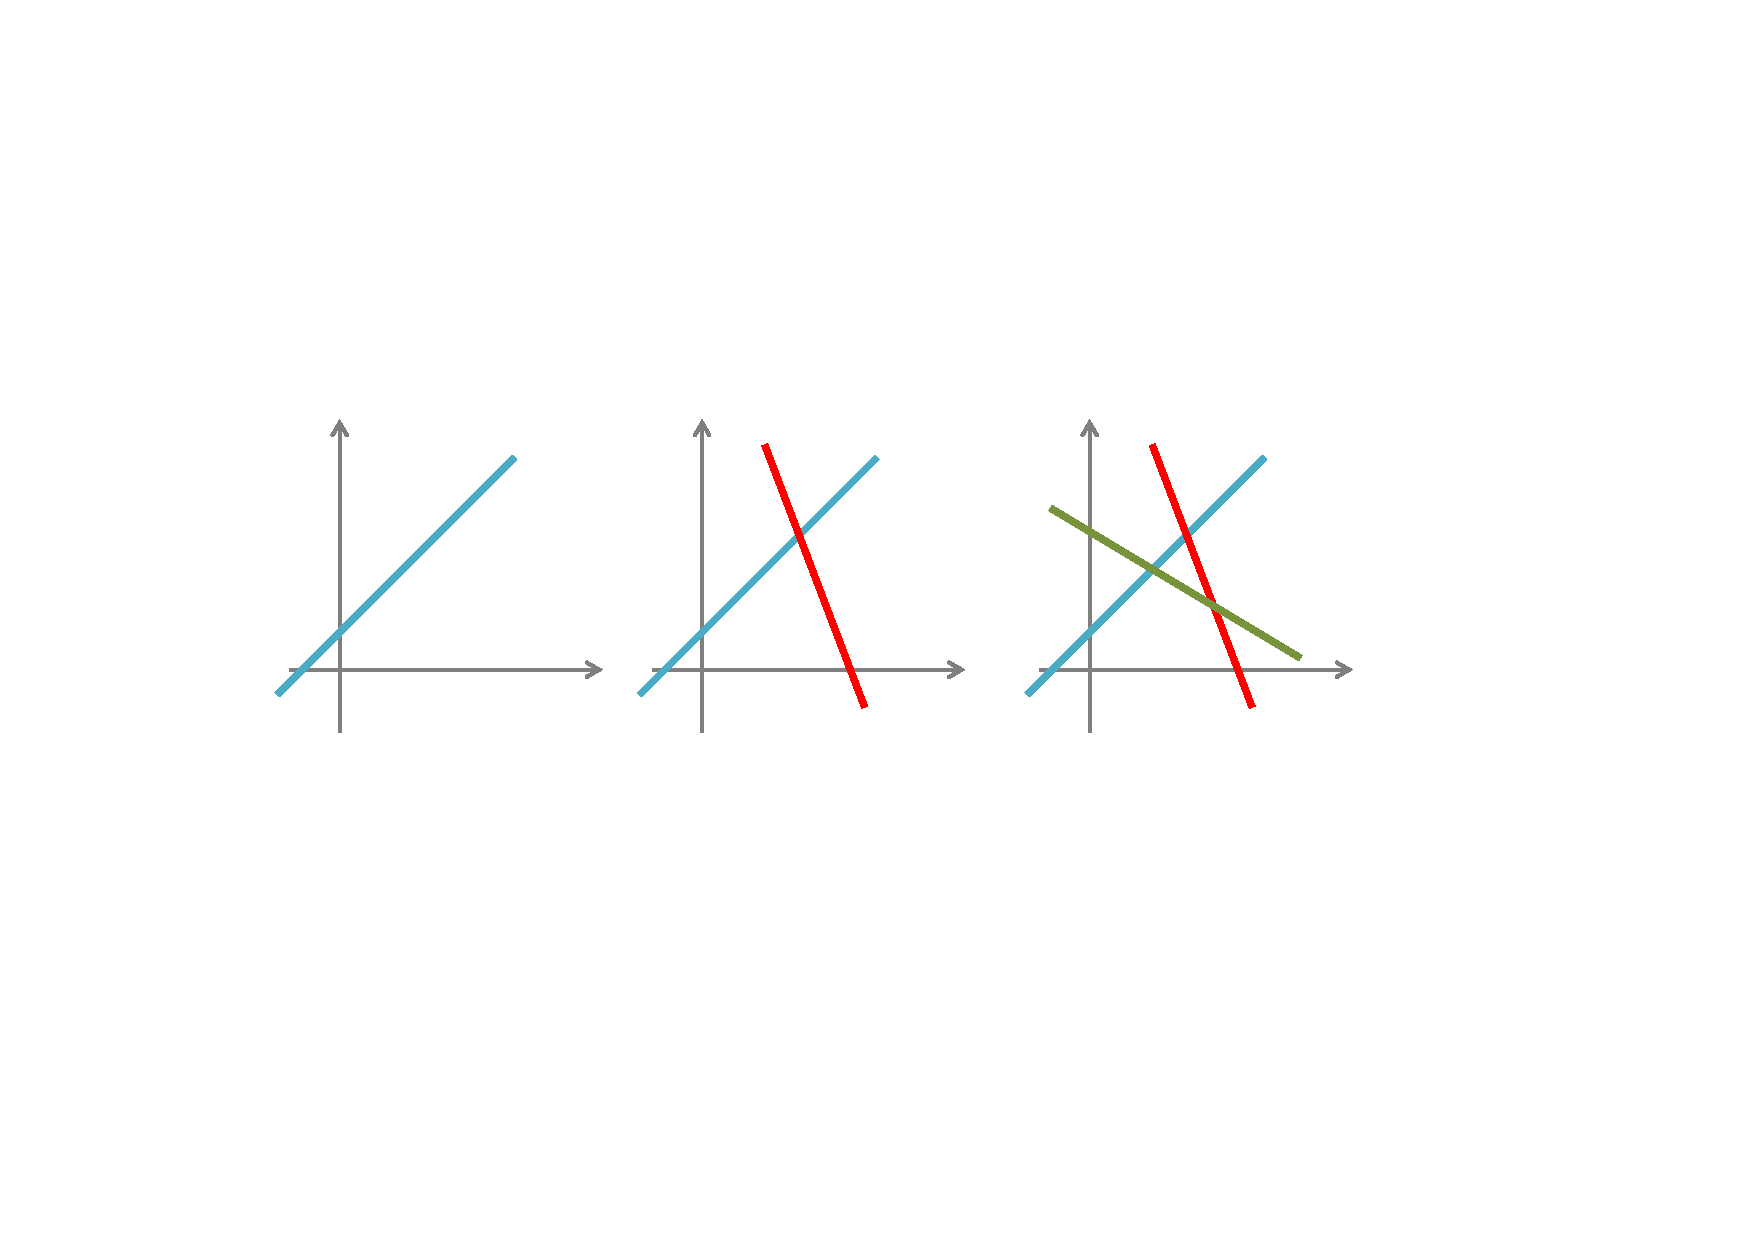
\includegraphics[trim = 40mm 90mm 65mm 60mm, clip, width=\textwidth]{./img/eqs-geometry-1}
\end{center}

\begin{columns}
\column{.3\textwidth}
\onslide<2->
\beq{
\begin{array}{lrr}
\textrm{\#vars} &=& 2\\
\textrm{\#eqs} &=& 1\\
\textrm{\#sols} &=& \infty\\
\end{array}
}

\column{.3\textwidth}
\onslide<3->
\beq{
\begin{array}{rrr}
\textrm{\#vars} &=& 2\\
\textrm{\#eqs} &=& 2\\
\textrm{\#sols} &=& 1\\
\end{array}
}

\column{.3\textwidth}
\onslide<4>
\beq{
\begin{array}{rrr}
\textrm{\#vars} &=& 2\\
\textrm{\#eqs} &=& 3\\
\textrm{\#sols} &=& 0\\
\end{array}
}
\end{columns}

\end{frame}

%%%%%%%%%%%%%%%%%%

\begin{frame}
\frametitle{A simple exercise}

How many \black{unknowns} (aka variables)?

\vspace{.2cm}

How many \black{equations}?

\vspace{.2cm}

How many \black{solutions}?

\begin{center}
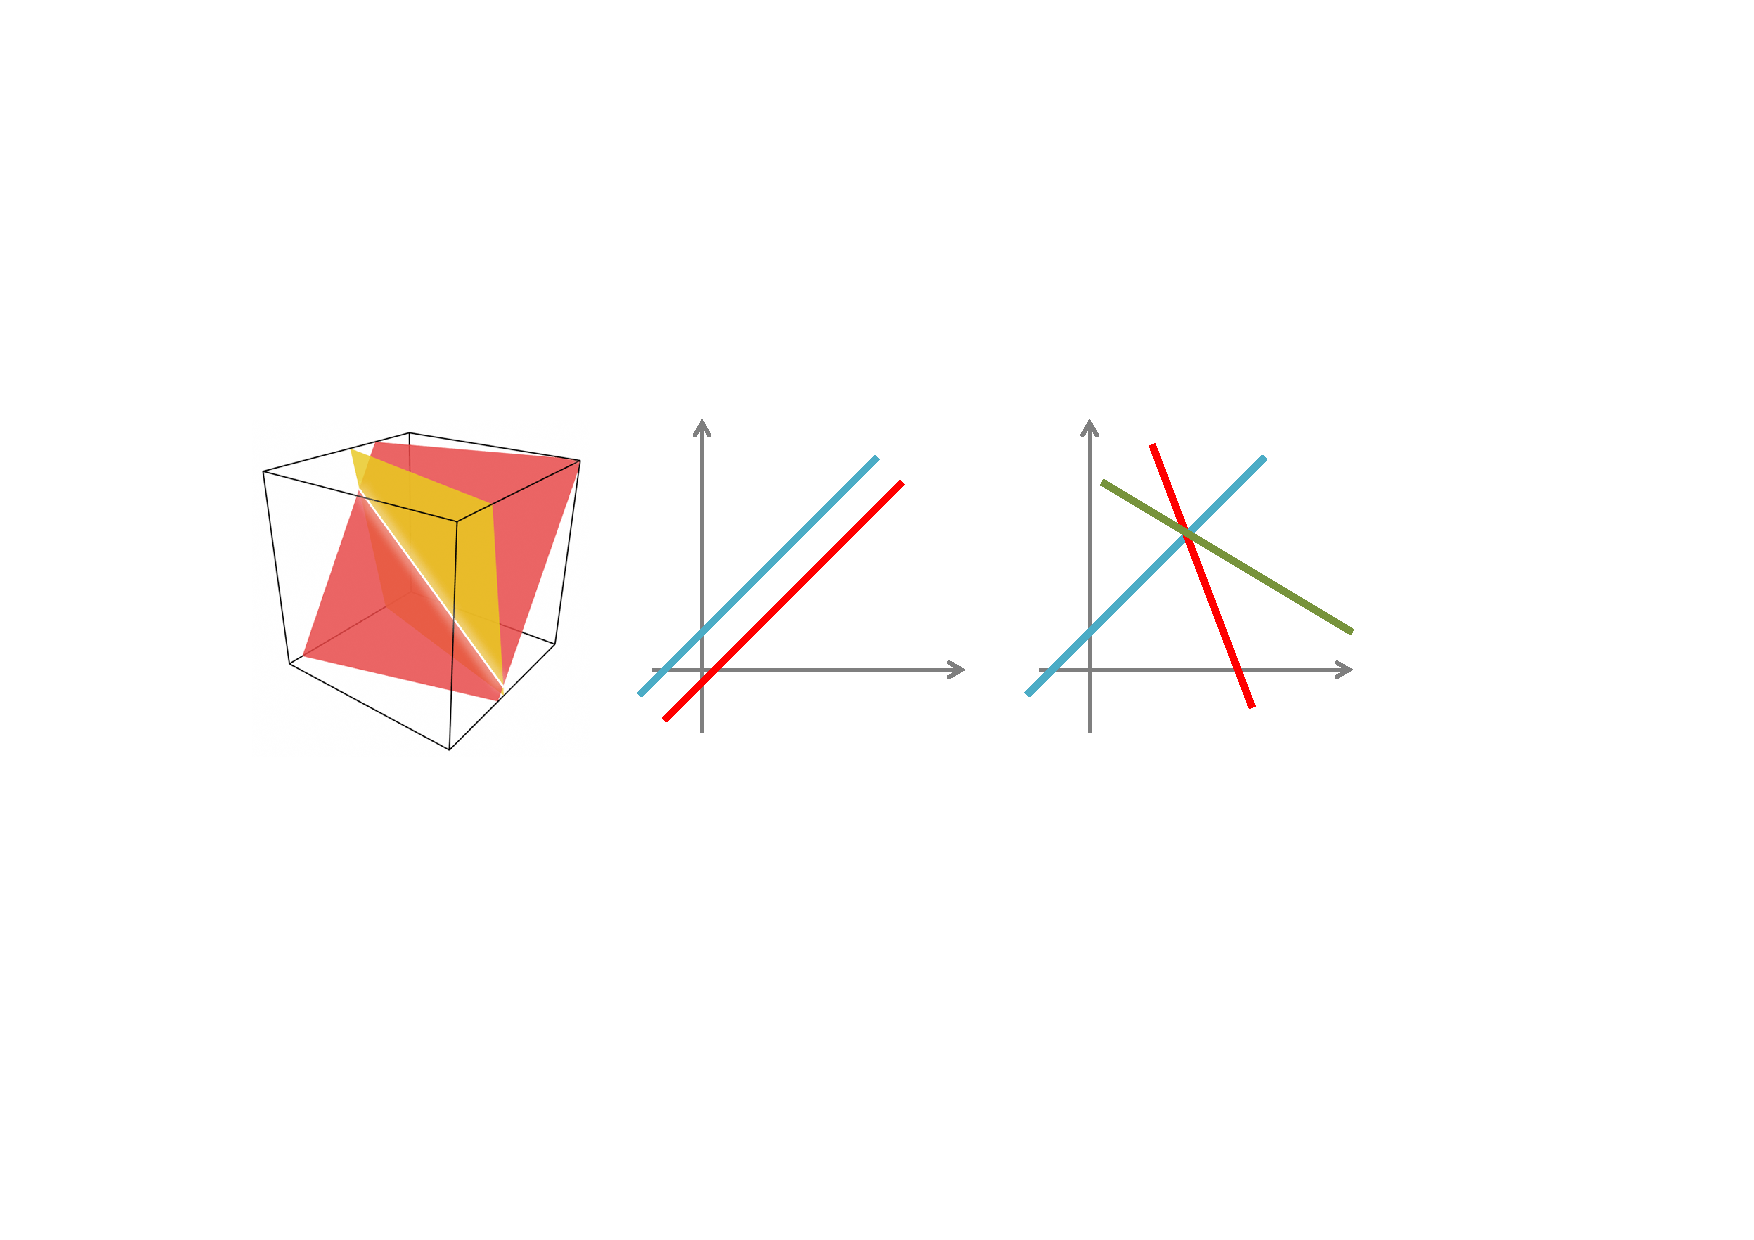
\includegraphics[trim = 40mm 85mm 65mm 60mm, clip, width=\textwidth]{./img/eqs-geometry-2}
\end{center}

\begin{columns}
\column{.3\textwidth}
\onslide<2->
\beq{
\begin{array}{lrr}
\textrm{\#vars} &=& 3\\
\textrm{\#eqs} &=& 2\\
\textrm{\#sols} &=& \infty\\
\end{array}
}

\column{.3\textwidth}
\onslide<3->
\beq{
\begin{array}{rrr}
\textrm{\#vars} &=& 2\\
\textrm{\#eqs} &=& 2\\
\textrm{\#sols} &=& 0\\
\end{array}
}

\column{.3\textwidth}
\onslide<4>
\beq{
\begin{array}{rrr}
\textrm{\#vars} &=& 2\\
\textrm{\#eqs} &=& 3\\
\textrm{\#sols} &=& 1\\
\end{array}
}
\end{columns}

\end{frame}






%%%%%%%%%%%%%%%%%%%%%%% MATRICES AND LINEAR INDEPENDENCE

\section{Linear independence}
\subsection*{}
%%%%%%%%%%%%%%%%%%

\begin{frame}
\frametitle{Elimination rapidly becomes cumbersome}

What are the values of $x_1$, $x_2$, $x_3$, $x_4$, $x_5$, $x_6$, $x_7$?

\beq{
\begin{array}{ccr}
-5x_1 + 2x_2 + 8x_3 + 4x_4 + 7x_5 - 6x_7 &=& 4\\
-x_1 + 3x_2 + 6x_3 - 7x_4 - 3x_5 + 8x_6 - 5x_7 &=& 0\\
9x_1 - 2x_2 - 8x_3 + 3x_4 + 4x_5 + 2x_6 + 7x_7 &=& -1\\
x_1 - 3x_2 - 5x_3 - 6x_5 + 2x_6 - 9x_7 &=& -8\\
9y - 3z + 5x_4 - 9x_5 + 7x_6 &=& 3\\
-5x_1 - 9x_2 + 3x_3 + 4x_4 + 5x_5 + 6x_6 - 6x_7 &=& -9\\
7x_2 - 7x_3 + 8x_4 + x_6+ 9x_7 &=& -8\\
\end{array}
}

\end{frame}


\begin{frame}
\frametitle{Matrix picture}

\beq{
\underbrace{\left[
\begin{array}{rrrrrrrr}
-5 & 2 & 8 & 4 & 7 & 0 & -6\\
-1 & 3 & 6 & -7 & -3 & 8 & -5\\
9 & -2 & -8 & 3 & 4 & 2 & 7\\
1 & -3 & -5 & 0 & -6 & 2 & -9\\
0 & 9 & -3 & 5 & -9 & 7 & 0\\
-5 & -9 & 3 & 4 & 5 & 6 & -6\\
0 & 7 & -7 & 8 & 0 & 1 & 9\\
\end{array}\right]}_{\A}
\underbrace{\left[
\begin{array}{r}
     x_1\\
     x_2\\
     x_3\\
    x_4\\
    x_5\\
    x_6\\
    x_7\\
\end{array}
\right]}_{\x}
=\underbrace{\left[
\begin{array}{r}
     4\\
     0\\
    -1\\
    -8\\
     3\\
    -9\\
    -8\\
\end{array}
\right]}_{\b}
}

In \emph{matrix} notation:

\beq{
\A\x = \b
}

Where $\black{\A}$ is a $\black{7x7}$ \emph{coefficient matrix}, $\black{\x}$ is $\black{7x1}$, and $\black{\b}$ is $\black{7x1}$.


\end{frame}

%%%%%%%%%%%%%%%%%%

\begin{frame}
\frametitle{Matrix multiplication}

How do we multiply a matrix $\black{\A}$ by a vector $\black{\x}$?

\beq{
\left[
\begin{array}{rr}
2 & 5\\
1 & 3
\end{array}
\right]
\left[
\begin{array}{r}
1\\
2
\end{array}
\right]=?
}

\onslide<2->
\underline{Method 1:} take the \emph{dot product} of each row of $\black{\A}$ with vector $\black{\x}$:

\beq{
\left[
\begin{array}{rr}
2 & 5\\
1 & 3
\end{array}
\right]
\left[
\begin{array}{r}
1\\
2
\end{array}
\right]=
\left[
\begin{array}{ccc}
2\cdot 1 &+& 5\cdot 2\\
1\cdot 1 &+& 3\cdot 2
\end{array}
\right]=
\left[
\begin{array}{c}
12\\
7
\end{array}
\right]
}

\onslide<3>
\underline{Method 2:} think of the entries of $\black{\x}$ as the coefficients of a linear combination of two column vectors:

\beq{
\left[
\begin{array}{rr}
2 & 5\\
1 & 3
\end{array}
\right]
\left[
\begin{array}{r}
1\\
2
\end{array}
\right]=
1\left[
\begin{array}{c}
2\\
1
\end{array}
\right]+
2\left[
\begin{array}{c}
5\\
3
\end{array}
\right]=
\left[
\begin{array}{c}
12\\
7
\end{array}
\right]
}


\end{frame}

%%%%%%%%%%%%%%%%%%

\begin{frame}
\frametitle{Linear independence}

Recall our simple system of two linear equations:


\beq{
\begin{array}{ccc}
2x - y & = & 0\\
-x + 2y& = &3
\end{array}
}

which can be written in matrix form:

\beq{
\underbrace{\left[
\begin{array}{rr}
2 & -1\\
-1 & 2\\
\end{array}
\right]}_{\A}
\left[
\begin{array}{c}
x\\ 
y
\end{array}
\right] = \underbrace{\left[
\begin{array}{c}
0\\ 
3
\end{array}
\right]}_{\b}
}

Thinking $\black{x}$ and $\black{y}$ as coefficients in a linear combination of vectors:

\beq{
x\underbrace{\left[
\begin{array}{r}
2\\
-1
\end{array}
\right]}_{\a_1}+y
\underbrace{\left[
\begin{array}{r}
-1\\
2
\end{array}
\right]}_{\a_2} = \underbrace{\left[
\begin{array}{c}
0\\ 
3
\end{array}
\right]}_{\b}
}

\end{frame}


%%%%%%%%%%%%%%%%%%

\begin{frame}
\frametitle{Linear independence}

\beq{
x\underbrace{\left[
\begin{array}{r}
2\\
-1
\end{array}
\right]}_{\a_1}+y
\underbrace{\left[
\begin{array}{r}
-1\\
2
\end{array}
\right]}_{\a_2} = \underbrace{\left[
\begin{array}{c}
0\\ 
3
\end{array}
\right]}_{\b}
}

We know that this system of equations has one unique solution. But, is that true for any $\black{\b}$?

\onslide<2>
\vspace{1cm}
\emph{YES} because $\black{\a_1}$ and $\black{\a_2}$ are \emph{linearly independent} and thus the linear combinations of $\black{\a_1}$ and $\black{\a_2}$ fill the whole $\black{2}$-dimensional plane.

\end{frame}

%%%%%%%%%%%%%%%%%%

\begin{frame}
\frametitle{Linear independence}

A set of vectors $\black{\v_1}$, $\black{\v_2}$, $\black{\v_3}$ are \emph{linearly independent} if any of them cannot be written as a linear combination of the other two, i.e.

\beq{
\v_i \neq \alpha\v_j + \beta\v_k \qquad  \forall \alpha \quad \forall \beta \quad \forall i\neq j \neq k
}

\vspace{2cm}

\tiny{\black{Note:} If you don't know what a linear combination is, \href{http://en.wikipedia.org/wiki/Linear_combination}{click here}.}


\end{frame}

%%%%%%%%%%%%%%%%%%

\begin{frame}
\frametitle{Linear independence}
For any system of $\black{m}$ linear equations with $\black{n}$ unknowns:

\beq{
\left[ 
\begin{array}{ccc}
a_{11} & \cdots & a_{1n}\\
\vdots & \ddots & \vdots\\
a_{m1} &\cdots & a_{mn}
\end{array}
\right]\left[
\begin{array}{c}
x_1\\
\vdots\\
x_n
\end{array}
\right] = 
\left[
\begin{array}{c}
b_1\\
\vdots\\
b_m
\end{array}
\right]
}

\vspace{.5cm}
Then

\vspace{.5cm}

\begin{tabular}{llcl}
$\black{\A}$ has $\black{k = n < m}$ & LI columns & $\Rightarrow$ & Unique or no solution\\
$\black{\A}$ has $\black{k = m = n}$ & LI columns & $\Rightarrow$ & Unique solution\\
$\black{\A}$ has $\black{k = m < n}$ & LI columns & $\Rightarrow$ & $\infty$ solutions
\end{tabular}

\vspace{.5cm}

$\black{\A}$ can have at most $m$ linearly independent columns. Why?

\end{frame}


%%%%%%%%%%%%%%%%%%

\begin{frame}
\frametitle{Why should I care?}

In Neuroimaging (and in many other fields of Science) you are rarely able to measure directly the processes of interest.

\vspace{.5cm}
Instead, you often measure a linear combination of your hidden (or latent) variables of interest. 

\vspace{.5cm}
For instance, in EEG, we don't measure directly tiny neural currents in brain tissue, but the electric potentials that such currents generate at the scalp:

\beq{
\v = \A\x
}


where $\black{\x}$ is an $\black{n\times 1}$ vector with current values at $\black{n}$ brain locations, $\black{\v}$ is an $\black{m\times 1}$ vector of potentials at $\black{m}$ scalp locations, and $\black{\A}$ is an $\black{m\times n}$ \emph{leadfield matrix}.


\end{frame}


%%%%%%%%%%%%%%%%%%%%%%%%%%%%%%%%%%% INVERSE
\section{Inverse}
\subsection*{}


\begin{frame}
\frametitle{Back to the large system of equations}

\beq{
\underbrace{\left[
\begin{array}{rrrrrrrr}
-5 & 2 & 8 & 4 & 7 & 0 & -6\\
-1 & 3 & 6 & -7 & -3 & 8 & -5\\
9 & -2 & -8 & 3 & 4 & 2 & 7\\
1 & -3 & -5 & 0 & -6 & 2 & -9\\
0 & 9 & -3 & 5 & -9 & 7 & 0\\
-5 & -9 & 3 & 4 & 5 & 6 & -6\\
0 & 7 & -7 & 8 & 0 & 1 & 9\\
\end{array}\right]}_{\A}
\underbrace{\left[
\begin{array}{r}
     x_1\\
     x_2\\
     x_3\\
    x_4\\
    x_5\\
    x_6\\
    x_7\\
\end{array}
\right]}_{\x}
=\underbrace{\left[
\begin{array}{r}
     4\\
     0\\
    -1\\
    -8\\
     3\\
    -9\\
    -8\\
\end{array}
\right]}_{\b}
}

In \emph{matrix} notation:

\beq{
\A\x = \b
}

\onslide<2>
\alert{How do we get $\x$?}

\end{frame}

%%%%%%%%%%%%%%%%%%

\begin{frame}
\frametitle{Inverse matrix}


For any square matrix $\black{\A}$, its inverse (if it exists) is defined as the matrix $\black{\A^{-1}}$ such that:

\beq{
\A\A^{-1}=\I
}

where $\black{\I}$ is the \emph{identity matrix}, i.e. a matrix with ones in the diagonal and zeroes everywhere else. If $\black{\A}$ is $\black{4\times 4}$ then:

\beq{
\I_{4} = \left[
\begin{array}{cccc}
1 & 0 & 0 & 0\\
0 & 1 & 0 & 0\\
0 & 0 & 1 & 0\\
0 & 0 & 0 & 1
\end{array}
\right]
}

\vspace{.5cm}
If $\black{\A^{-1}}$ exists, then it is unique.

\vspace{.5cm}
If we knew $\black{\A^{-1}}$, how could we use it to solve $\black{\A\x=\b}$ ?

\end{frame}


%%%%%%%%%%%%%%%%%%

\begin{frame}
\frametitle{Invertible systems / Invertible matrices}

\tiny{\black{Note:} Realize that $\black{\M\I=\I\M=\M}$ and $\black{\b\I=\I\b=\b}$ for any matrix $\black{\M}$ and for any vector $\black{\b}$}

\vspace{.5cm}

\small

Given a system of equations $\black{\A\x=\b}$ with $\black{\A}$ square then: 

\beq{
\x = \A^{-1}\b
}

if $\black{\A}$ is invertible. 

\vspace{.5cm}
Notice that this holds for any $\black{\b}$!

\vspace{.5cm}
What condition do you think $\black{\A}$ must fulfill to be invertible?

\end{frame}

%%%%%%%%%%%%%%%%%%

\begin{frame}[fragile]
\frametitle{How do we know if a matrix is invertible?}

Any non-singular matrix is invertible. 

\vspace{.5cm}
A square matrix is \emph{singular} if not all of its columns are linearly independent. You can check this in MATLAB using:

\vspace{.5cm}
\color{black}\verb|det(A)|\color{gray}

\vspace{.5cm}
If the determinant of $\black{\A}$ is zero, then $\black{\A}$ is singular.


\end{frame}


%%%%%%%%%%%%%%%%%%

\begin{frame}[fragile]
\frametitle{How do we calculate the inverse of a matrix?}

There are several techniques. A common one is the so-called \emph{Gauss-Jordan elimination}.

\vspace{.5cm}

In MATLAB you can simply do:

\vspace{.5cm}

\color{black}
\verb|inv(A)|
\color{gray}

\end{frame}


%%%%%%%%%%%%%%%%%%%%%%%%%%%%%%%%%%% LEAST-SQUARES and Minimum norm
\section{LS and MN solutions}
\subsection*{}


\begin{frame}
\frametitle{What about non-square matrices?}

\vspace{.5cm}
Recall:

\beq{
\left[ 
\begin{array}{ccc}
a_{11} & \cdots & a_{1n}\\
\vdots & \ddots & \vdots\\
a_{m1} &\cdots & a_{mn}
\end{array}
\right]\left[
\begin{array}{c}
x_1\\
\vdots\\
x_n
\end{array}
\right] = 
\left[
\begin{array}{c}
b_1\\
\vdots\\
b_m
\end{array}
\right]
}

\vspace{.5cm}
Then

\vspace{.5cm}

\begin{tabular}{llcl}
$\black{\A}$ has $\black{k = n < m}$ & LI columns & $\Rightarrow$ & Unique or no solution\\
$\black{\A}$ has $\black{k = m < n}$ & LI columns & $\Rightarrow$ & $\infty$ solutions
\end{tabular}

\end{frame}

%%%%%%%%%%%%%%%%%%

\begin{frame}[fragile]
\frametitle{Minimum norm solution for $m<n$}

An \emph{underdetermined} system with $\black{m=1}$, $\black{n=2}$:


\beq{
x - y = b \Rightarrow \left[\begin{array}{rr}
1 & -1\\
\end{array}
\right]
\left[ 
\begin{array}{c}
x\\
y
\end{array}
\right] = b
 }

\begin{overprint}
\onslide<1>
\begin{center}
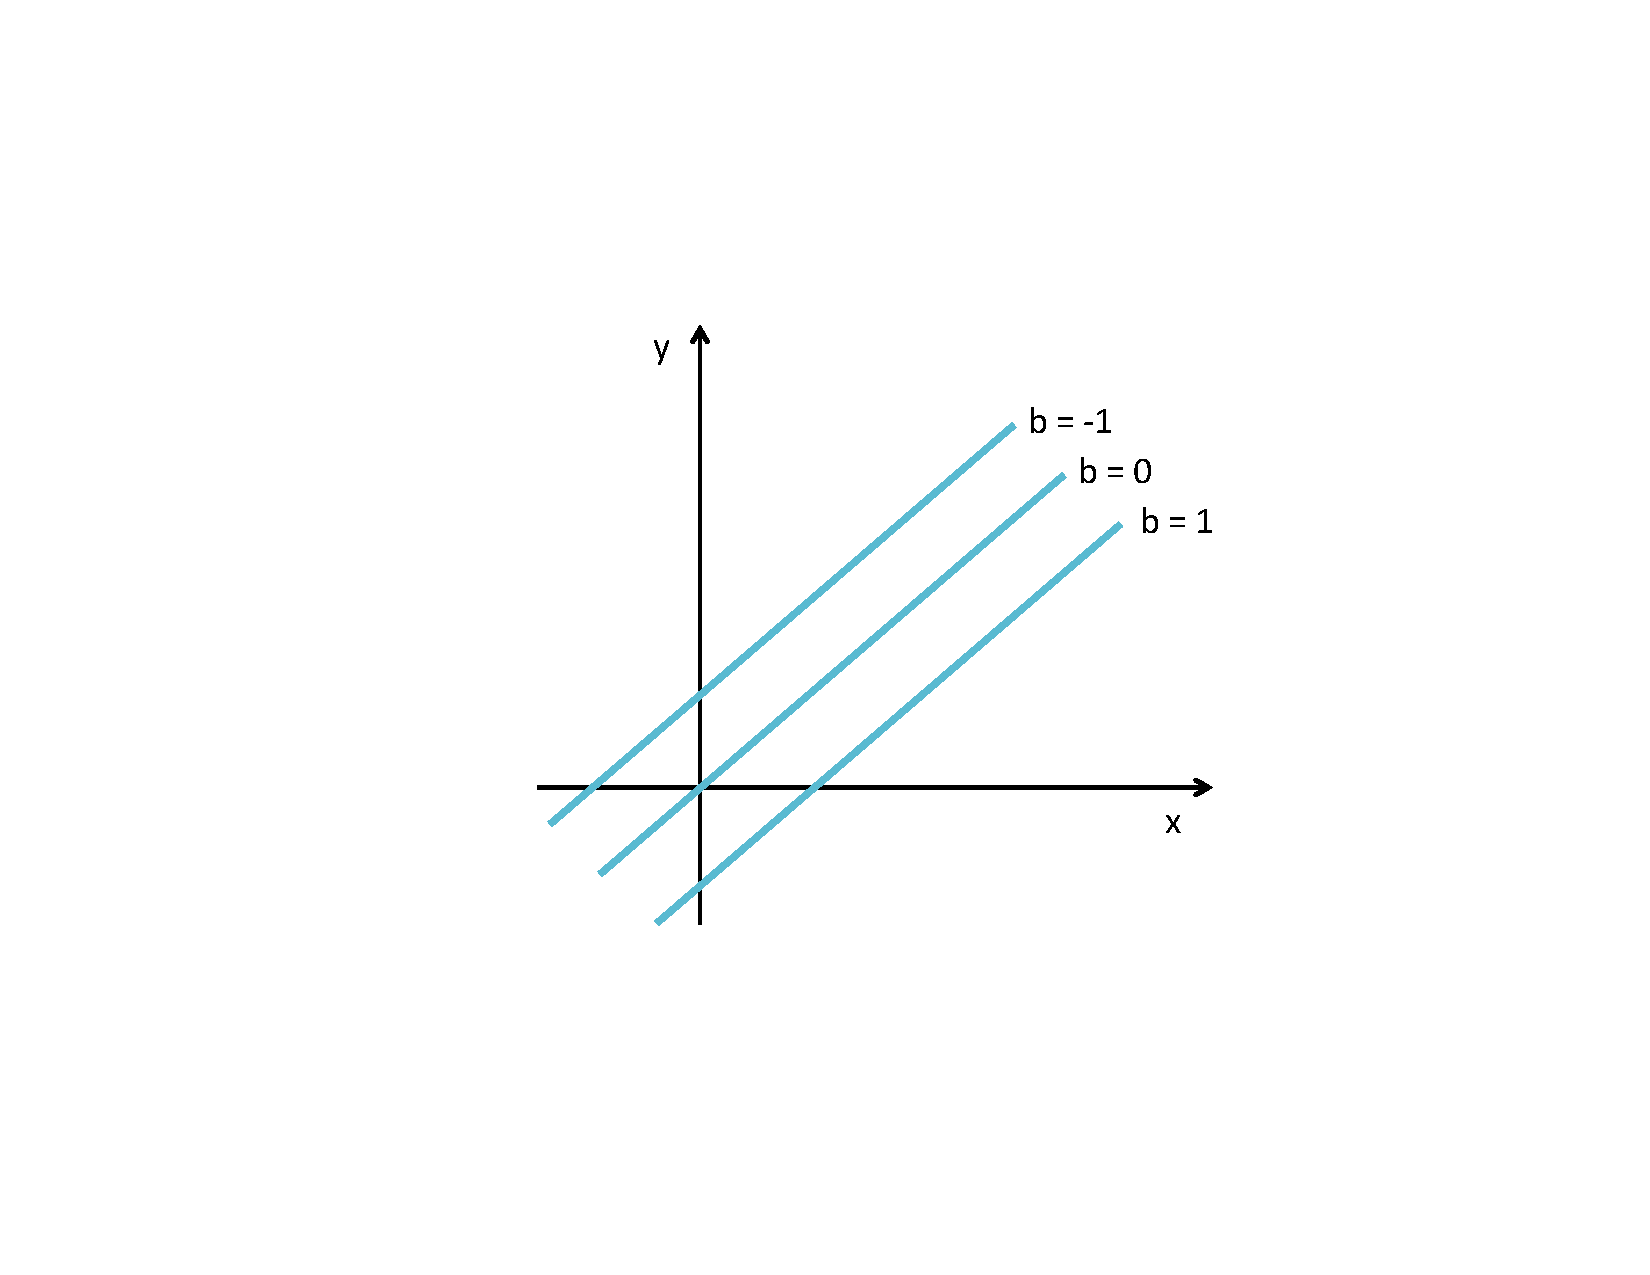
\includegraphics[trim = 40mm 65mm 65mm 50mm, clip, width=.7\textwidth]{./img/min-norm-1}
\end{center}

\onslide<2>
\begin{center}
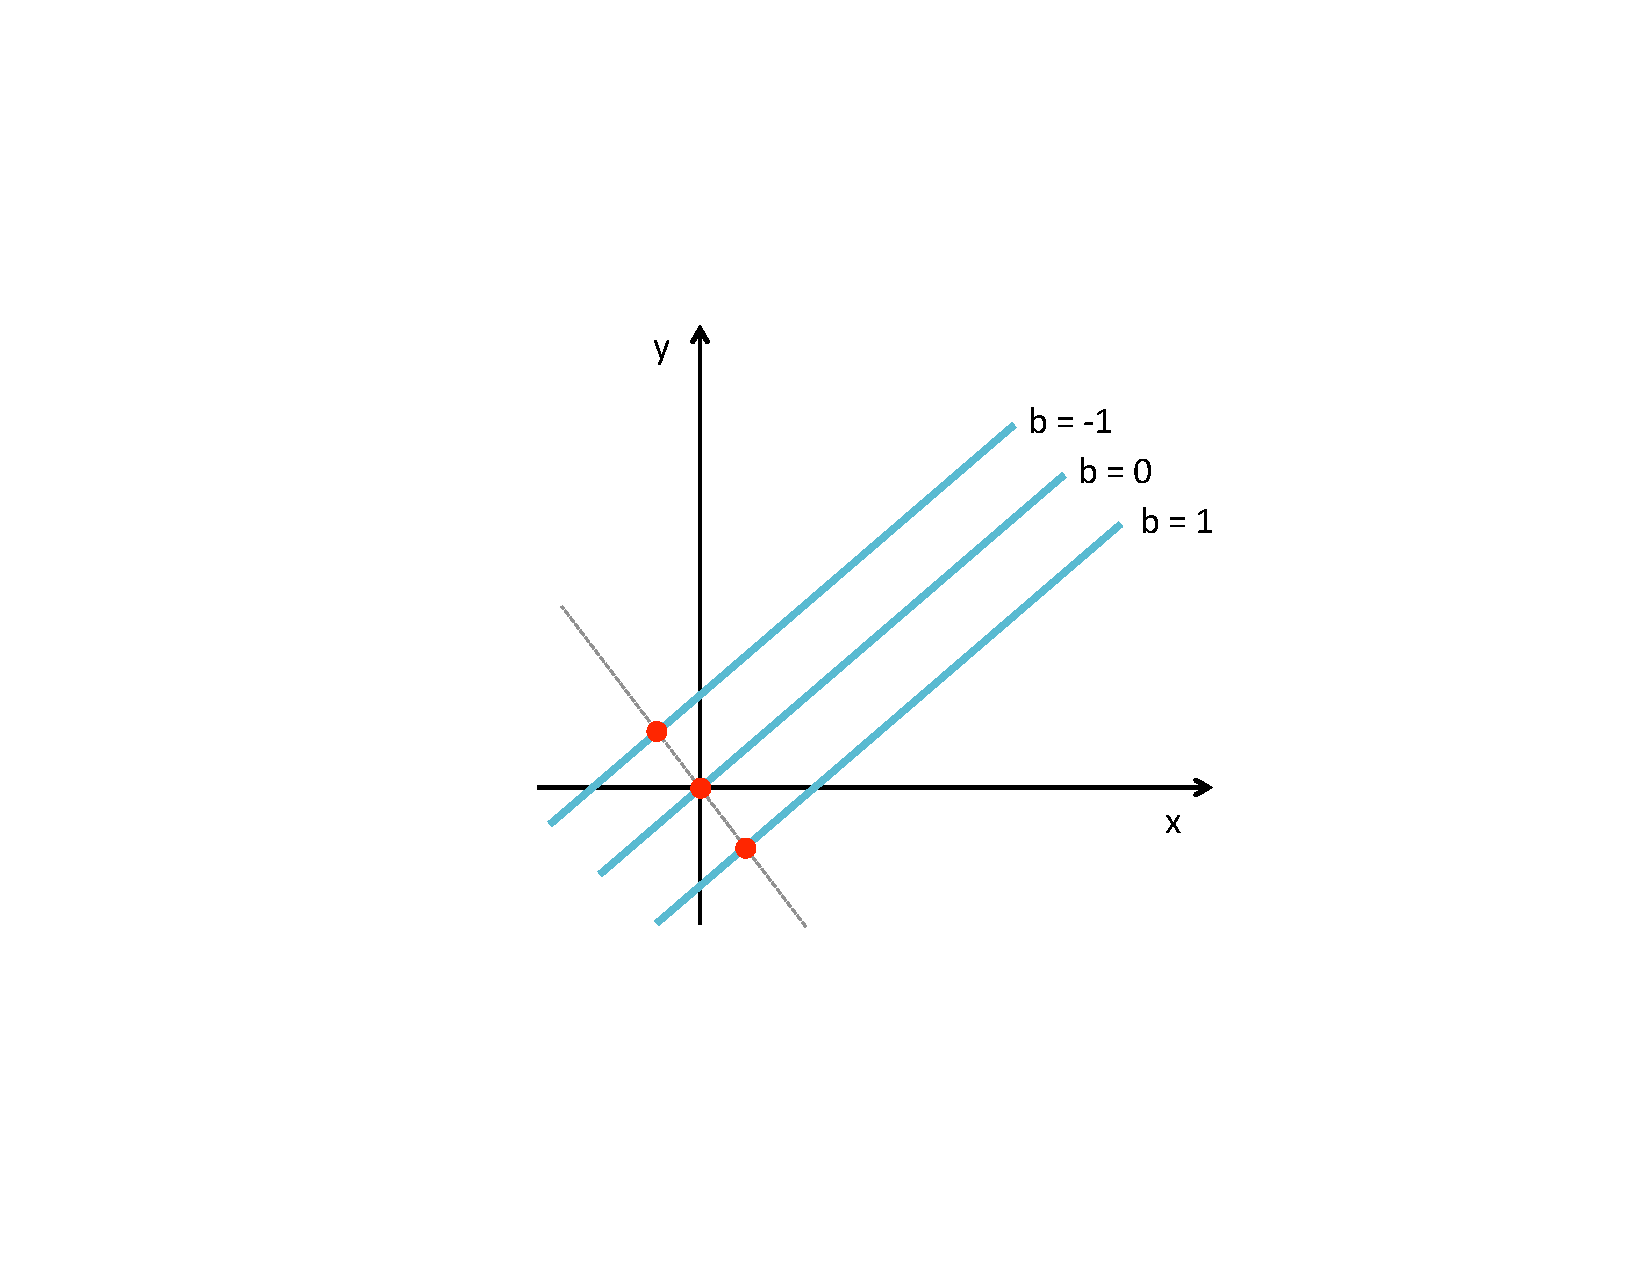
\includegraphics[trim = 40mm 65mm 65mm 50mm, clip, width=.7\textwidth]{./img/min-norm-2}
\end{center}
\vspace{.2cm}
Solution closest to the origin: The \emph{minimum norm} solution.
\end{overprint}

\end{frame}

%%%%%%%%%%%%%%%%%%

\begin{frame}[fragile]
\frametitle{Least squares solution for $m>n$}

An \emph{overdetermined} system with $\black{m=3}$, $\black{n=2}$:


\beq{
\begin{array}{rrr}
x + y   &=& 2 \\
2x - y  &=& 0\\
x - 2y  &=& 0
\end{array}
\Rightarrow \left[\begin{array}{rr}
1 & 1 \\
2 & -1 \\
1 & -2
\end{array}
\right]
\left[ 
\begin{array}{c}
x\\
y
\end{array}
\right] =  
\left[
\begin{array}{c}
2\\
0\\
0
\end{array}
\right]
}

\begin{overprint}
\onslide<1>
\begin{center}
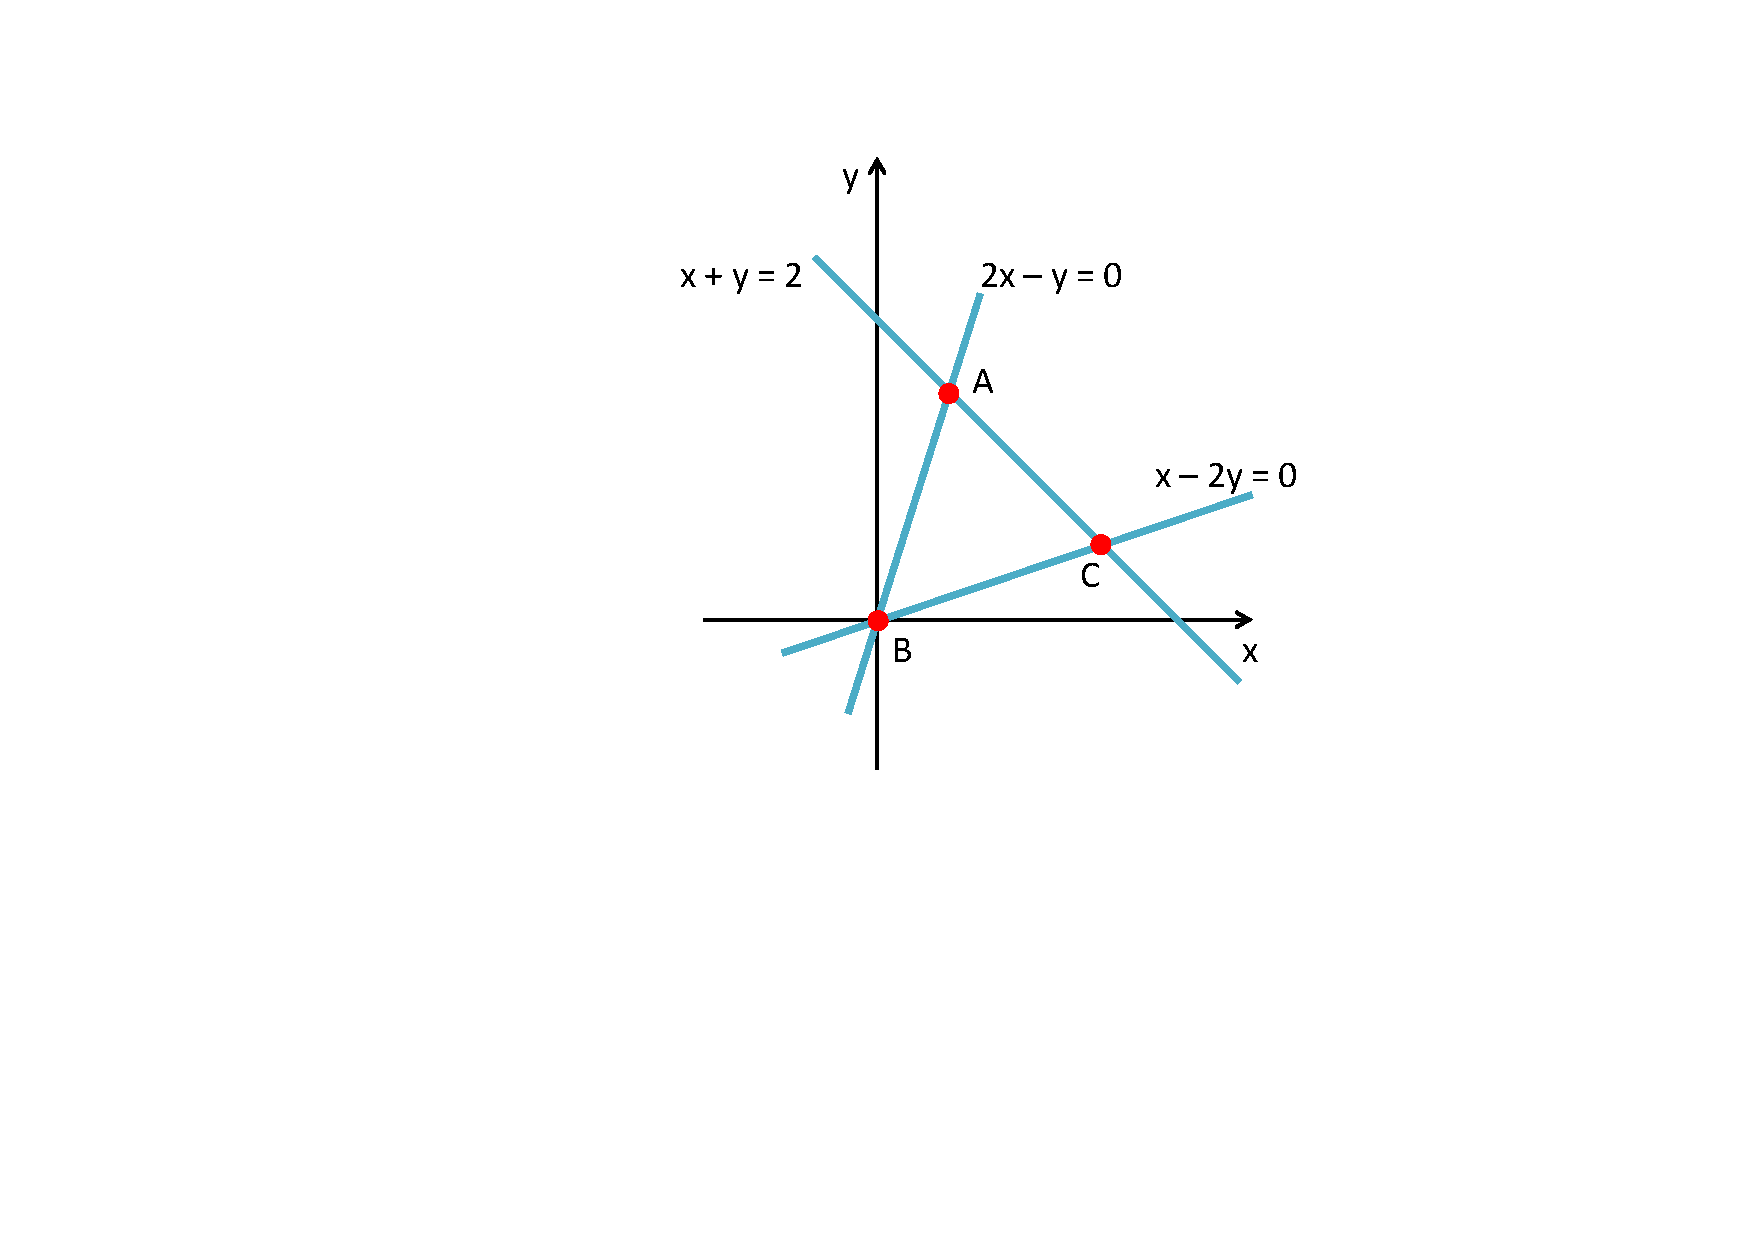
\includegraphics[trim = 80mm 90mm 60mm 20mm, clip, width=.6\textwidth]{./img/overdetermined-1}
\end{center}

\onslide<2>
\begin{center}
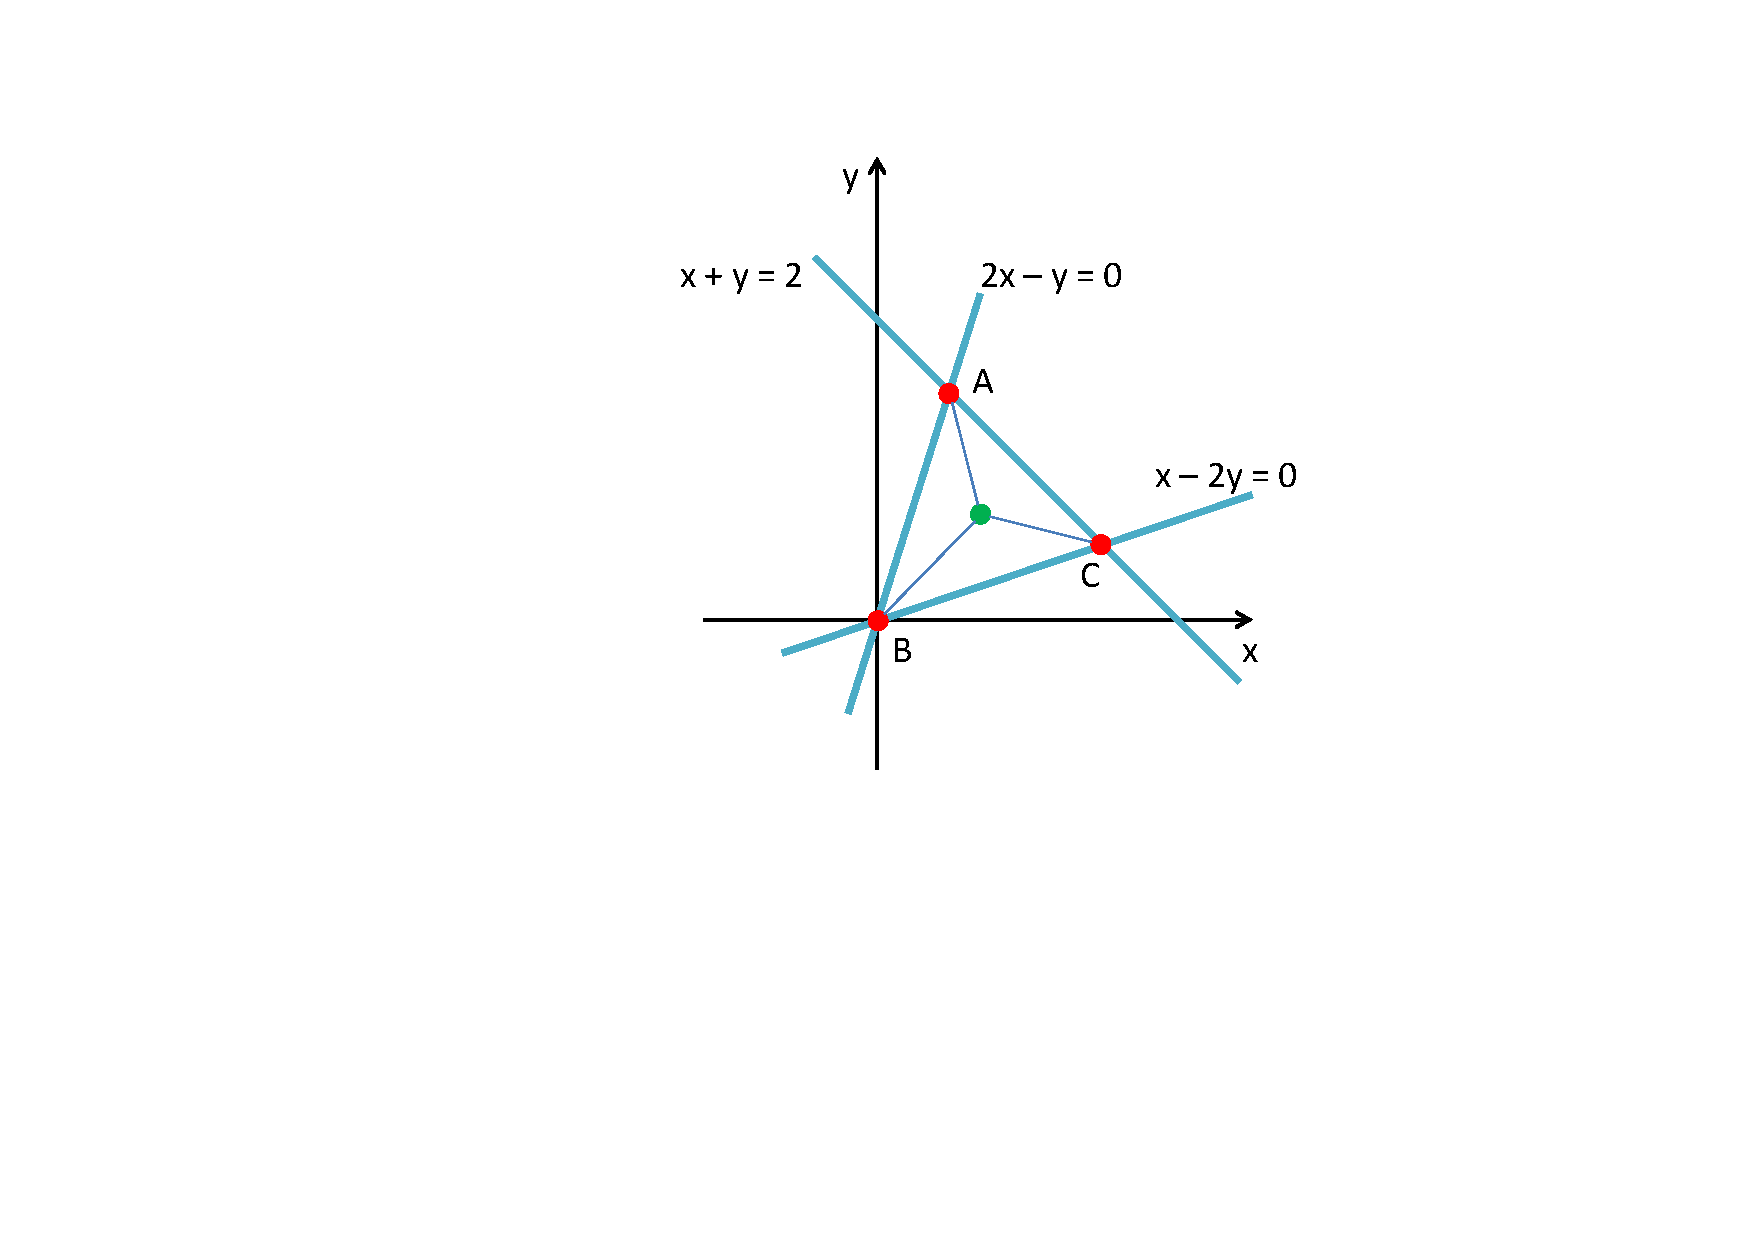
\includegraphics[trim = 80mm 90mm 60mm 20mm, clip, width=.6\textwidth]{./img/overdetermined-2}
\end{center}

Minimize Least Squared Error (LSE): The \emph{least squares} solution.

\end{overprint}

\end{frame}



%%%%%%%%%%%%%%%%%%

\begin{frame}
\frametitle{Pseudoinverse}

Given a linear system of $\black{m}$ equations and $\black{n}$ unknowns $\black{\A\x = \b}$ then, if the columns of $\black{\A}$ are linearly independent:

\beq{
\hat{\x} = \A^+\b
}

with $\black{\hat{\x}}$ being:

\begin{itemize}
\item The Least Squares solution if $\black{m > n}$
\item The Minimum Norm solution if $\black{m < n}$
\item The exact solution if $\black{m=n}$
\end{itemize}

\vspace{.5cm}
$\black{\A^+}$ is the \emph{pseudoinverse} of $\black{\A}$, and can be easily obtained as:

\beq{
\A^+ = \left(\A^T\A\right)^{-1}\A^T
}

\tiny{\black{Note:} $\black{\A^T}$ denotes the transpose of matrix $\black{\A}$. See \href{http://en.wikipedia.org/wiki/Transpose}{wikipedia.}}


\end{frame}



%%%%%%%%%%%%%%%%%

\begin{frame}[fragile]
\frametitle{The pseudoinverse is just the inverse for $m=n$}

For square matrices, the pseudoinverse reduces to the inverse:

\beq{
\A^+ = \left(\A^T\A\right)^{-1}\A^T = \A^{-1}\left(\A^T\right)^{-1}\A^T =  \A^{-1}
}

\vspace{.5cm}
In MATLAB: \color{black}\verb|pinv(A)|\color{gray}

\vspace{.5cm}
But, what if $\black{\A}$ has linearly dependent columns?

\vspace{.5cm}
Then neither $\black{\A}$ nor $\black{\left(\A^T\A\right)}$ are invertible, i.e. we cannot solve the linear system.

\onslide<2>
\vspace{.5cm}
\alert{So, ... should we just give up?}

\end{frame}


%%%%%%%%%%%%%%%%%

\section{Regularization}
\subsection*{}

\begin{frame}[fragile]
\frametitle{Regularization}

When $\black{\A}$ has linearly dependent columns the linear system is said to be \emph{ill-conditioned} and cannot be solved. However, we may still find the solution of a \emph{regularized} version of the original system of linear equations. That is, instead of using:


\beq{
\hat{\x} = \A^+\b		\qquad \textrm{with}\quad \A^+ = \left(\A^T\A\right)^{-1}\A^T
}

we are forced to use something like:

\beq{
\hat{\x}_R = \A^+_{\Gammam}\b		\qquad \textrm{with}\quad \A^+_{\Gammam}= \left(\A^T\A + \Gammam^T\Gammam\right)^{-1}\A^T
}

for some suitably chosen regularization matrix $\black{\Gammam}$.

\end{frame}

%%%%%%%%%%%%%%%%% HOW DOES REGULARIZATION AFFECT THE SOLUTION?

\begin{frame}[fragile]
\frametitle{How does regularization affect the solution?}

Regularization allows a numerical solution for \emph{ill-conditioned} linear systems, at the expense of giving preference to certain solutions.

\vspace{.5cm}
If regularization is based on valid a-priori information on the true solution, it enables a numerical solution of an otherwise unsolvable \emph{inverse problem}.

\vspace{.5cm}
If a too harsh regularization is used or if it is based on wrong a-priori information, it can lead to a numerically stable but completely wrong solution.


\end{frame}


%%%%%%%%%%%%%%%%% THE CONDITIONING OF A MATRIX IS NOT ALWAY CLEAR-CUT

\begin{frame}[fragile]
\frametitle{The conditioning of a matrix is not always clear cut}

Sometimes it is:

\beq{
\A = 
\left[
	\begin{array}{rrr}
	9 & 9 & 0\\
	2 & 5 & -3\\
	9 & 8 & 1\\
	\end{array}
\right]
}

Notice that $\black{\a_3=\a_1-\a_2}$. Indeed, in MATLAB we get:

\begin{verbatim}
>> rank(A)

ans =

     2
\end{verbatim}

\tiny{\black{Note:} MATLAB's command \verb|rank| tells us the number of linearly independent columns of a matrix. You can also check that the determinant of this matrix is zero using command \verb|det|.} 

\end{frame}

%%%%%%%%%%%%%%%%% THE CONDITIONING OF A MATRIX IS NOT ALWAY CLEAR-CUT (cont'd)

\begin{frame}[fragile]
\frametitle{The conditioning of a matrix is not always clear cut}

But most often it is not:

\beq{
\B = 
\left[
	\begin{array}{rrr}
	9 & 9 & 0.001\\
	2 & 5 & -3.001\\
	9 & 8 & 1.001\\
	\end{array}
\right]
}

In MATLAB we get:

\begin{verbatim}
>> rank(B)

ans =

     3
\end{verbatim}

Can we conclude that $\black{\A}$  is ill-conditioned but $\black{\B}$ is not?


\end{frame}


%%%%%%%%%%%%%%%%%  THE CONDITION NUMBER OF A MATRIX
\begin{frame}[fragile]
\frametitle{The condition number of a matrix}

Matrix conditioning is characterized by the condition number:

\color{black}
\begin{verbatim}
>> cond(A)
ans =

   1.8076e+16
   
>> cond(B)
ans =

   1.1644e+05
\end{verbatim}

\color{gray}

The condition number ranges from \black{1} (the identity matrix) to \black{Inf} (any matrix with linearly dependent columns, e.g. $\black{\A}$).
\end{frame}


%%%%%%%%%%%%%%%%%  WHAT DOES THE CONDITION NUMBER TELLS US?
\begin{frame}[fragile]
\frametitle{What does the condition number tells us?}

From \black{\href{http://en.wikipedia.org/wiki/Condition\_number}{Wikipedia}}:

\vspace{.3cm}

\textit{\small{''the condition number of a function with respect to an argument measures the worst case of how much the function can change in proportion to small changes in the argument"}} 

\onslide<2->

\vspace{.2cm}
The functions we are interested in are:

\beq{
\A\x = \b
}

\beq{
\x = \A^{-1}\b
}

Where $\black{\x}$ might be the tiny brain currents in the brain tissue, and $\black{\b}$ might be the associated scalp potentials.

\end{frame}

%%%%%%%%%%%%%%%%%  CONCLUSIONS ABOUT THE COND NUMBER
\begin{frame}[fragile]
\frametitle{What are the implications for M/EEG source modeling?}

If the matrix that maps brain currents to scalp potentials is ill-conditioned then:

\vspace{.4cm}

\begin{itemize}

\item \black{Tiny changes in the brain currents (e.g. simply due to the stochastic nature of brain activity) will produce large changes in the measured potentials}

\vspace{.2cm}

\item \black{Tiny changes in the measured scalp potentials (e.g. due to electrical noise) will lead to largely different inverse M/EEG solutions}

\end{itemize}

\end{frame}





%%%%%%%%%%%%%%%%%%%%%%% REFERENCES

\section{References}
\subsection*{}

\begin{frame}
\frametitle{References and Attribution}

\small

These slides are partially based on course materials available at MIT Open Courseware:

\vspace{.5cm}
\black{\url{http://ocw.mit.edu/courses/mathematics/18-06sc-linear-algebra-fall-2011/}}


\vspace{1cm}

Some images are from Wikipedia:

\vspace{.5cm}
\black{\url{http://en.wikipedia.org/wiki/System_of_linear_equations}}


\end{frame}

\end{document}
